%=========================================================================
% (c) 2014, 2015 Josef Lusticky

\chapter{Analysis}
Basically, there are three important parts needed to perform network benchmarks at full 40 Gbit speeds -
a network interface card with 40Gb Ethernet support, a server compatible with the card and a packet generator.
A chosen distribution of the GNU/Linux operating system should contain a stable and
recent kernel that supports the 40 Gigabit Ethernet protocol and the network interface card.

%=========================================================================
% (c) 2014, 2015 Josef Lusticky

\section{Hardware and networking}\label{sec:setup-hardware}
Figure~\ref{fig:setup-supermicro-board} shows the block diagram of the Supermicro motherboard.
The Intel Xeon E5-2660 v2 processors were plugged into the CPU sockets.
The Mellanox ConnectX-3 EN adpater was plugged into the PCIE 3.0 x8 Upper slot,
which is part of the {\it{WIO}} block.
The PCI-Express links are directly connected to the CPU~1 only.
\begin{figure}
	\centering
	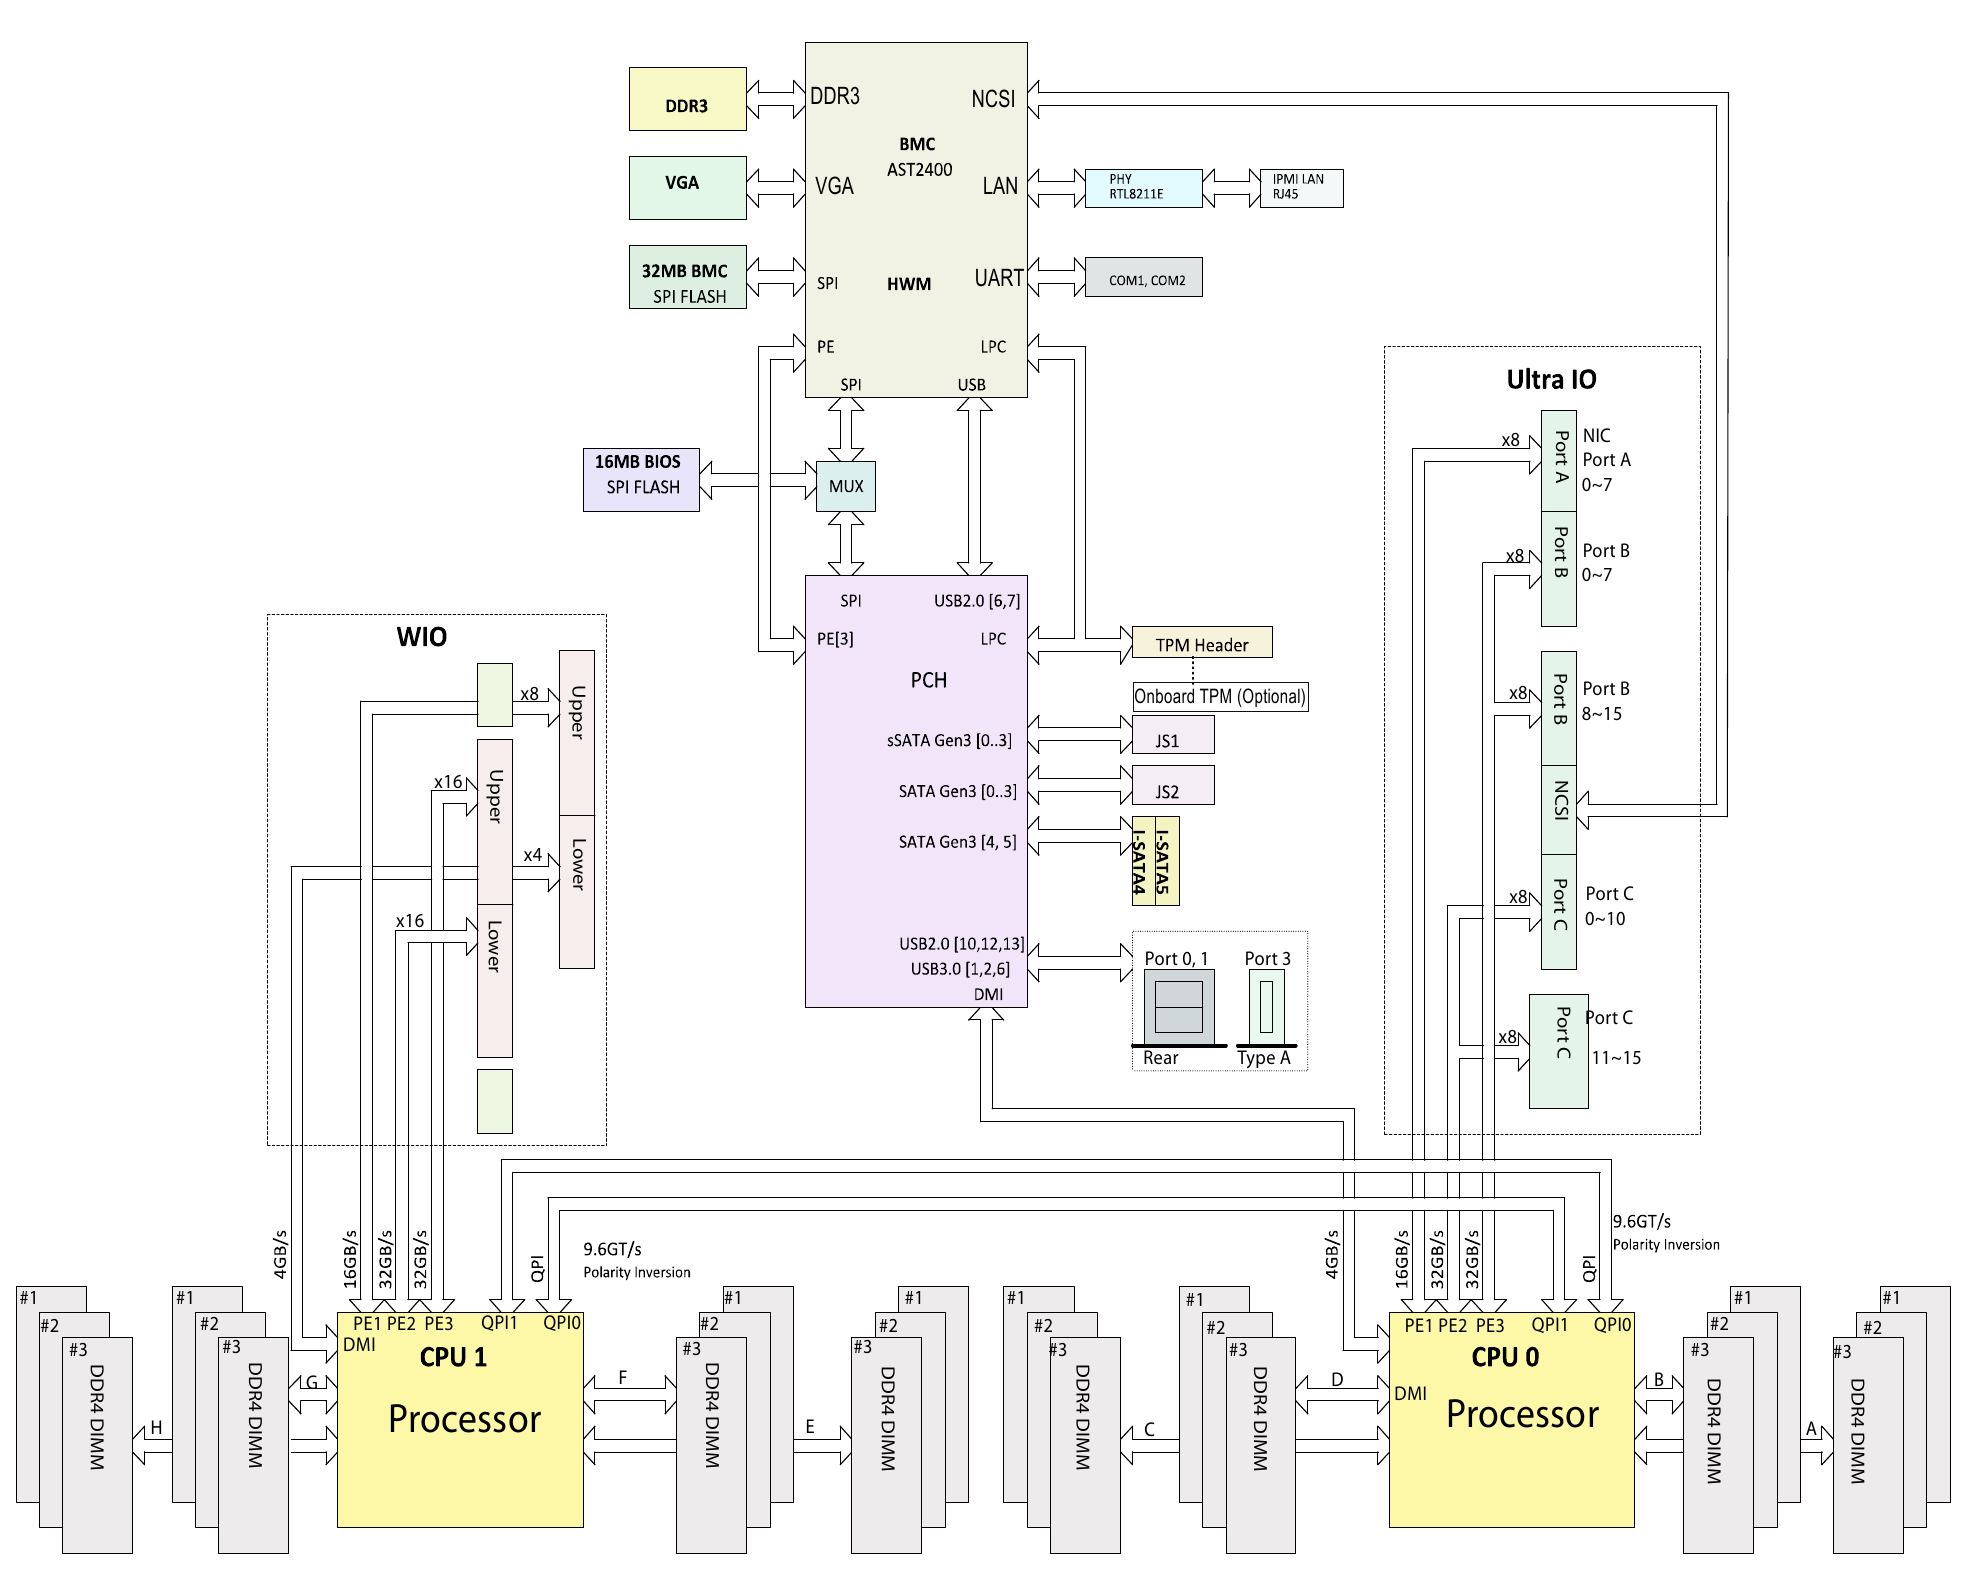
\includegraphics[width=15cm,keepaspectratio]{fig/supermicro-x10drui.png}
	\caption{Supermicro motherboard's block diagram}
	\label{fig:setup-supermicro-board}
\end{figure}

The server was put to the same rack as the Spirent hardware generator.
A pair of 40GBASE-SR4 multimode fiber cables with QSPF connectors
was used to connect Spirent with the Mellanox ConnectX-3 EN adapter.

IPv4 addresses from 192.0.2.0/24 (TEST-NET-1) block were assigned~\cite{rfc5737}.
IPv6 addresses from 2001:db8::/32 range were assigned.
Addresses within these blocks should not appear on the public Internet~\cite{rfc3849}.
Figure~\ref{fig:addressing-scheme} shows the addressing scheme used for the measurements.
\begin{figure}[H]
	\centering
	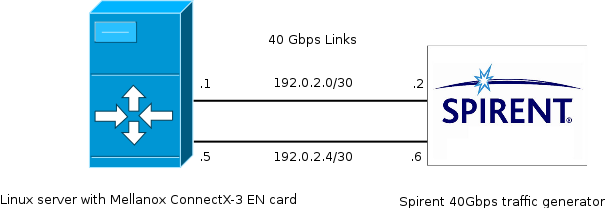
\includegraphics[width=13.5cm,keepaspectratio]{fig/net-setup.png}
	\caption{Addressing scheme}
	\label{fig:addressing-scheme}
\end{figure}



%Enable IPv4 packet forwarding:
%echo 1 > /proc/sys/net/ipv4/ip\_forward


%ip neigh add 1.0.0.2 lladdr f4:52:14:5e:6c:71 dev enp6s0d1
%ip neigh add 2.0.0.2 lladdr f4:52:14:5e:6c:70 dev enp6s0

%ip addr add 1.0.0.1/24 broadcast 1.0.0.255 dev enp6s0d1
%ip addr add 2.0.0.1/24 broadcast 2.0.0.255 dev enp6s0


%Load BGP routes:
%\begin{lstlisting}
%Basic info: size of leaf: 40 bytes, size of tnode: 40 bytes.
%Main:
        %Aver depth:     2.43
        %Max depth:      8
        %Leaves:         503308
        %Prefixes:       538739
        %Internal nodes: 114430
          %1: 58725  2: 26171  3: 14808  4: 7316  5: 4239  6: 2103  7: 1065  8: 2  17: 1
        %Pointers: 995798
%Null ptrs: 378061
%Total size: 61373  kB
%\end{lstlisting}


%=========================================================================
% (c) 2014, 2015 Josef Lusticky

\section{Software and firmware}
Base CentOS 7 was installed on the server.
The operating system features Linux kernel based on version 3.10 -
the installed version is 3.10.0-123.20.1.el7.x86\_64.
The operating system was updated with all updates available as of 1st May 2015.
The upstream kernel version 4.0.2 was additionally installed from the ELRepo repository~\cite{elrepo-kernel-ml}.

The Linux kernel detects the Mellanox ConnectX-3 EN card automatically and loads the mlx4\_core and mlx4\_en module.
The mlx4\_core module prints the detected PCI-Express link parameters to the kernel's message buffer.
The buffer can be viewed using the {\it{dmesg}} utility and its partial output is shown bellow:
\begin{lstlisting}[language=TeX]
mlx4_core 0000:06:00.0: PCIe link speed is 8.0GT/s, device supports 8.0GT/s
mlx4_core 0000:06:00.0: PCIe link width is x8, device supports x8
\end{lstlisting}
The mlx4\_core module further registers interrupts and prints the assigned IRQ numbers for each queue
to the kernel's message buffer:
\begin{lstlisting}[language=TeX]
mlx4_core 0000:06:00.0: irq 61 for MSI/MSI-X
mlx4_core 0000:06:00.0: irq 62 for MSI/MSI-X
...
mlx4_core 0000:06:00.0: irq 90 for MSI/MSI-X
\end{lstlisting}

The driver uses either MSI or MSI-X feature of the PCI-Express bus, as described in section~\ref{sec:40gbe-throughput}.
The MSI-X feature is used automatically if the system supports it, otherwise the adapter uses MSI.
The {\it{lspci -vv}} command can be used to check whether MSI-X is used.
Listing~\ref{lst:setup-lspci} shows partial output of lspci for the Mellanox ConnectX-3 EN adapter.
The MSI-X capability is followed by an Enable flag which is followed with either "+" (enabled)
or "-" (disabled).
Listing~\ref{lst:setup-lspci} shows that the system supports MSI-X and the adapter is configured to use it.
\begin{lstlisting}[language=TeX,label={lst:setup-lspci},caption={Partial output of lspci -vv for Mellanox ConnectX-3 EN}]
06:00.0 Ethernet controller: Mellanox Technologies MT27500 Family [ConnectX-3]
		...
		Capabilities: [9c] MSI-X: Enable+ Count=128 Masked-
				...
				LnkCap: Port #8, Speed 8GT/s, Width x8, ASPM L0s, Exit Latency L0s unlimited, L1 unlimited
				...
\end{lstlisting}

Apart from the NIC driver, the Mellanox ConnectX-3 adapter uses its own proprietary firmware.
The firmware was updated to version 2.32.5100, which is the latest version available as of 10th January 2015.
The firmware is not part of the Linux kernel and its update procedure is described in appendix~\ref{app:firmware}.


%=========================================================================
% (c) 2014, 2015 Josef Lusticky

\section{Benchmarking methodology}\label{sec:analysis-metodology}
Procedures described by RFC~2544 can be used to measure routing performance of the Linux kernel.
RFC~2544 specifies the benchmarking methodology for network interconnect devices.
The ideal way to implement the series of tests described in RFC~2544 is to use a tester
with both transmitting and receiving ports.
Connections are made from the sending ports of the tester to the receiving ports of the
device under test (DUT) and from the sending ports of the DUT back to the tester~\cite{rfc2544}.
Figure~\ref{fig:analysis-rfc2544} shows the test implementation.

Since the tester both sends the test traffic and receives
it back, after the traffic has been forwarded by the DUT, the tester
can easily determine if all of the transmitted packets were received~\cite{rfc2544}.
The Spirent TestCenter Application provides statistics about transmitted and received frames,
which can be used for this purpose.
\begin{figure}
	\centering
	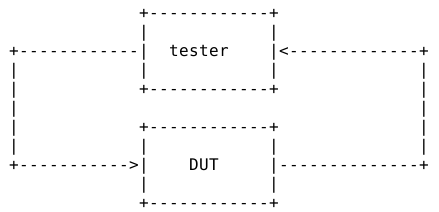
\includegraphics[width=9cm,keepaspectratio]{fig/rfc2544.png}
	\caption{RFC2544 test implementation (source:~\cite{rfc2544})}
	\label{fig:analysis-rfc2544}
\end{figure}

%=========================================================================
% (c) 2014, 2015 Josef Lusticky

\subsection{Traffic generation}\label{sub:analysis-metodology-generation}
The RFC~2544 specifies the following frame sizes to be used on Ethernet:
64, 128, 256, 512, 1024, 1280 and 1518~\cite{rfc2544}.
However, at least 66~B frame size must be used in case of transmitting UDP over IPv6 - the size of L2 header is 14,
the size of CRC is 4, the size of IPv6 header is 40 and the size of UDP header is 8.

In addition to the specified frame sizes, a custom frame size distribution can be defined for the purpose of
a real internet traffic simulation.
The Amsterdam Internet Exchange (AMS-IX) provides
statistics of the frame size distribution in the Internet traffic~\cite{amsix-frame-size}.
Figure~\ref{fig:analysis-amsix-frame-size} shows yearly frame size distribution provided by AMS-IX.
This distribution can be configured in the Spirent TestCenter Application, however,
to use the same iMix for both IPv4 and IPv6, the minimum frame size must be increased to 66 as described above.
To avoid an unfair packet scheduling by the server, all packets should be assigned the same Type of Service flag.

Unfortunately,
the provided Spirent TestCenter Application does not contain license to configure a device participating in TCP streaming.
This constraint could be workarounded by sending TCP packets with no flags set,
however such configuration is also not possible.
The generated TCP packets always contain TCP SYN flag,
which bypasses the Generic Receive Offload described in subsection~\ref{sub:linux-ingress-offloads}.
Therefore, the TCP packet processing is the same as in case of UDP.

The Spirent TestCenter Application allows to configure exact frame rate or bandwidth use.
The measurements should distinguish at least between 50~000 frames per second or 1\% of bandwidth use.
Each measurement takes 60~seconds and it is repeated 3 times.
If the kernel is able to forward all frames in at least one of the 3 measurements,
the measurement is successful.
This is to determine whether the kernel is able to forward such amount of traffic.
Some network unrelated tasks performed by the kernel may cause the inability to forward all frames,
such as gathering statistics, memory management, etc.

\begin{figure}
	\centering
	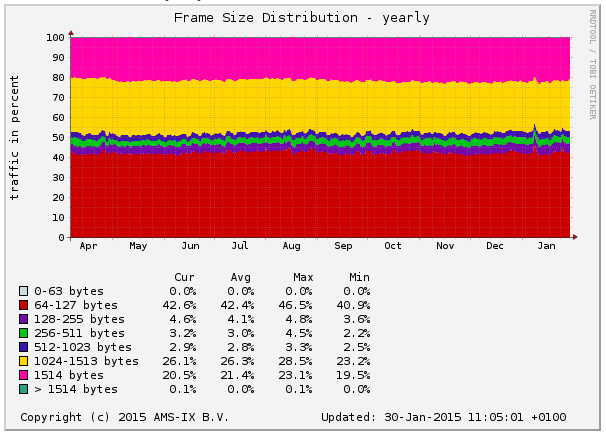
\includegraphics[width=14.5cm,keepaspectratio]{fig/amsix.png}
	\caption{Yearly frame size distribution at AMS-IX (source:~\cite{amsix-frame-size})}
	\label{fig:analysis-amsix-frame-size}
\end{figure}


%=========================================================================
% (c) 2014, 2015 Josef Lusticky

\subsection{Statistics collection}
The Spirent TestCenter Application is able to display counters of transmitted and received frames on each interface.
The counters can be used to determine whether all of the transmitted packets on one interface were received
on the other interface and hence successfully forwarded by the server.
Unfortunately, the provided Spirent TestCenter Application contains no licence to perform the RFC 2544 throughput test
automatically, so the measurements must be configured manually in the Spirent TestCenter application.
The manual configuration consists of configuring the transmit rate, observing the packet counters and comparing their values.
If the server forwards packets without a single loss, the transmit rate can be increased and the test repeated.
%Otherwise, the transmit rate must be decreased.

The proc filesystem provides access to several statistics as well.
The network statistics exported via proc filesystem can be found in the /proc/net directory.
The files in this directory are read-only and cannot be manipulated using the sysctl utility.
There are 2 important files for the measurements - the {\it{fib\_trie}} and {\it{fib\_triestat}}.
The {\it{fib\_trie}} file exports the kernel's Forwarding Information Base overview.
The file describes both the Main and Local FIBs, as described in section~\ref{sec:linux-routing}.
The {\it{fib\_triestat}} file exports metadata of the FIB trie structures,
such as average depth, maximum depth, number of leaves, etc~\cite{kernel-source}.

The CPU utilisation can be observed using the perf utility,
which can be found in the tools/perf directory of the Linux kernel source code.
Although perf is included in the Linux kernel source code,
it must be installed separately on most GNU/Linux distributions, including CentOS~7.
To obtain additional statistics, such as PCI-Express utilisation or memory utilisation,
the Intel Performance Counter Monitor (PCM)\footnote{\url{https://software.intel.com/en-us/articles/intel-performance-counter-monitor-a-better-way-to-measure-cpu-utilization}}
can be used.
The PCM package is not included in the official CentOS~7 repository,
but it can be compiled directly from the source code.
Non-maskable interrupt watchdog must be disabled
in order to run Intel PCM.
The non-maskable interrupt watchdog can be disabled by writing "0" to the /proc/sys/kernel/nmi\_watchdog file.



%=========================================================================
% (c) 2014, 2015 Josef Lusticky

\section{Software settings}\label{sec:analysis-settings}
The CentOS 7 operating system features various components that influence forwarding performance.
To measure a pure routing performance of the Linux kernel,
the Netfilter and SELinux components should be disabled.
If disabling the netfilter is not appropriate, the iptables utility must be used to configure netfilter to allow forwarding,
because the default rules do not allow packet forwarding.
SELinux in the CentOS~7 operating system uses enforcing policy by default.
Similarly to netfilter, the SELinux component should be disabled to prevent performance decrease.
Influence of both the components on forwarding performance can be measured.

The Linux kernel features dynamic CPU frequency scaling.
The CPUFreq governors are policies that decide what frequency should be used.
The CPUfreq governor {\it{performance}} should be used during the measurements, as it sets the CPU statically to the
highest frequency avaliable~\cite{cpufreq-governors}. %, which is 2.6~GHz in case of Intel Xeon E5-2630 v2.

Packet processing by the Linux kernel can be configured in different ways.
To change the Linux kernel compile-time configuration, the kernel must be recompiled.
The CentOS~7 kernel provides a fair amount of features that could break existing setups when disabled.
The default kernel compile-time configuration does not have to provide the best routing performance,
however, it is usually used in most scenarious and hence its benchmark results are of interests for most people.
The features configured during compile-time of the Linux kernel introduce
just a negligible overhead when they are not used.
For example, the MULTIPLE\_IP\_TABLES support is enabled in the CentOS 7 distribution kernel, however,
since the measurements presented in this thesis use no policy routing,
the FIB lookup principle described in section~\ref{sec:linux-routing} is still performed.

Apart from compile-time options, the Linux kernel configuration can be changed during run-time.
The proc and sys filesystems provide access to the kernel variables that influence packet processing.
Tuning of these variables can provide significant amount of routing performance improvement when configured properly.

\subsection{Procfs settings}
The variables exported via procfs are accessible in CentOS~7 as read-write files in /proc.
The variables in the /proc/sys directory can be changed by the sysctl utility as well.
The files in the /proc/sys/net directory are of interest for the experiments.
This directory includes the following subdirectories:
\begin{itemize}
\item /proc/sys/net/ipv4 - variables influencing the IPv4 protocol settings
\item /proc/sys/net/ipv6 - variables influencing the IPv6 protocol settings
\item /proc/sys/net/netfilter - variables influencing the netfilter settings, not discussed in this thesis
\item /proc/sys/net/unix - variables influencing communication over unix sockets, not discussed in this thesis
\item /proc/sys/net/core - variables influencing low-level network settings, including parameters of NAPI, Low Latency Sockets, etc.
\end{itemize}

The most important setting for the routing performance measurements of the Linux kernel is IPv4 forwarding.
It can be enabled by writing "1" to the /proc/sys/net/ipv4/ip\_forward file.
This variable is special - its change resets all IPv4 configuration parameters to their default state~\cite{kernel-doc-ip-sysctl}.
The /proc/sys/net/ipv4/conf/{\it{ifname}}/forwarding file can be used
to further selectively enable or disable forwarding on a particular interface.
Historically, some of the files in /proc/sys/net/ipv4 also influence settings of L4 protocols.
Although these files are located in the ipv4 subdirectory, the L4 settings are independent on the underlying protocol.

Files in the ipv6 directory influence the IPv6 protocol settings only.
The IPv6 protocol is disabled in CentOS 7 on all interfaces by default.
The variable accessible via /proc/sys/net/ipv6/conf/all/disable\_ipv6 must be changed to "0" to
enable the IPv6 protocol on all interfaces.
Similarly, the /proc/sys/net/ipv6/conf/all/forwarding variable must changed to "1" to enable IPv6 forwarding on all interfaces.
Both settings can be changed on per-interface basis as well.

The /proc/sys/net/ipv4/route.max\_size sets the maximum number of IPv4 routes allowed in the kernel.
This is 2~147~483~647 by default in CentOS~7, which is enough for a full BGP table,
which contains approx.~538~000 prefixes at the time of writing. %TODO cite
The /proc/sys/net/ipv6/route.max\_size sets the maximum number of IPv6 routes allowed in the kernel.
This is 4096 by default in CentOS~7, which must be raised for the measurements involving BGP routes.
The number of IPv6 prefixes announced in the Internet is approx.~22~000 at the time of writing. %TODO cite

The source IPv4 address validation is enabled by default in CentOS 7.
This feature is called Reverse path filtering (rp\_filter) in the Linux kernel and it prevents IP spoofing.
However, it introduces additonal processing and thus it should be disabled during the experiments.
The rp\_filter can be disabled on a particular interface
by writing "0" to /proc/sys/net/ipv4/conf/{\it{ifname}}/rp\_filter~\cite{kernel-doc-ip-sysctl}.
The rp\_filter for IPv6 was implemented in the netfilter subsystem of the Linux kernel and
thus it can be configured by iptables~\cite{kernel-source}.

Files in core directory provide access to low-level variables of the networking code.
There are two parameters that influence NAPI processing.
The /proc/sys/net/core/dev\_weight file sets the maximum number of packets that a single device
can feed to the kernel in its {\it{poll()}} function.
The default value is 64 in CentOS 7.
This value can be increased to allow the device to feed more packets at once.
However, most of the drivers provide their own limit which cannot be overwritten unless the code of the driver is changed.
This is the case of the mlx4 driver as well~\cite{kernel-source}.
The /proc/sys/net/core/netdev\_budget file sets the
maximum number of packets taken from all interfaces by a single {\it{net\_rx\_action()}} run.
The interfaces which are registered to polling are
probed in a round-robin manner, as described in subsection~\ref{subsec:linux-ingress-napi}.
To allow the kernel to spend more time on packet processing, the netdev\_budget value can be increased.

Apart from settings, the proc filesystem provides access to several statistics as well.
The network statistics exported via proc filesystem can be found in the /proc/net directory.
The files in this directory are read-only and cannot be manipulated using the sysctl utility.
There are 2 important files for the measurements - the fib\_trie and fib\_triestat.
The fib\_trie file exports the kernel's Forwarding Information Base overview.
The file describes both the Main and Local FIBs, as described in section~\ref{sec:linux-routing}.
The fib\_triestat file exports metadata of the FIB trie structures,
such as average depth, maximum depth, number of leaves, etc.

\subsection{Sysfs settings}
Apart from the proc filesystem, the Linux kernel provides another virtual filesystem found in /sys.
Every interface is represented by a symlink in the /sys/class/net/ directory.
The symlinks point to the corresponding network device, which is represented as a directory in sysfs.

The scaling mechanisms described in section~\ref{sec:linux-scaling} can be set
using files exported in /sys/class/net/{\it{ifname}}/queues.
Each rx-{\it{xx}} subdirectory represents a single hardware receive queue.
The rx-{\it{xx}}/rps_cpus file can be used to set a mask of CPUs serving the particular queue.
Since the Mellanox ConnectX-3 NIC supports RSS, the RPS feature is disabled by default.

%XPS

The sysfs further exports information about loaded modules, including the parameters if a particular module takes any.
The /sys/modules/mxl4\_core/parameters directory contains parameters used by the mlx4\_core module.
The msi\_x parameter is set to 1 by default, which means attempt to use MSI-X.
The /sys/modules/mxl4\_en/parameters directory contains parameters used by the mlx4\_en module.
The udp\_rss parameter is set to 1 by default, which enables RSS for incoming UDP traffic.
There are more parameters taken by both modules, but they are not discussed in this thesis.
Further description of the parameters can be found
in the drivers/net/ethernet/mellanox/mlx4 directory of the Linux kernel source code~\cite{kernel-source}.

\subsection{Ethtool settings}
Ethernet devices can be also configured using ethtool.
Ethtool is a standard Linux utility for controlling network drivers and hardware, particularly for
wired Ethernet devices.
Supported offload features can be displayed using ethtool -{}-show-offload {\it{devname}}.
Listing~\ref{lst:analysis-ethtool-offload} shows output of ethtool -{}-show-offload eth0,
where eth0 is the Mellanox ConnectX-3 adpater.

\begin{lstlisting}[caption={Output of ethtool -{}-show-offload for Mellanox ConnectX3 adapter},label={lst:analysis-ethtool-offload}]
rx-checksumming: on
tx-checksumming: on
	tx-checksum-ipv4: on
	tx-checksum-ip-generic: off [fixed]
	tx-checksum-ipv6: on
	tx-checksum-fcoe-crc: off [fixed]
	tx-checksum-sctp: off [fixed]
scatter-gather: on
	tx-scatter-gather: on
	tx-scatter-gather-fraglist: off [fixed]
tcp-segmentation-offload: on
	tx-tcp-segmentation: on
	tx-tcp-ecn-segmentation: off [fixed]
	tx-tcp6-segmentation: on
udp-fragmentation-offload: off [fixed]
generic-segmentation-offload: on
generic-receive-offload: on
large-receive-offload: off [fixed]
rx-vlan-offload: on [fixed]
tx-vlan-offload: on [fixed]
ntuple-filters: off [fixed]
receive-hashing: on
highdma: on [fixed]
rx-vlan-filter: on [fixed]
vlan-challenged: off [fixed]
tx-lockless: off [fixed]
netns-local: off [fixed]
tx-gso-robust: off [fixed]
tx-fcoe-segmentation: off [fixed]
tx-gre-segmentation: off [fixed]
tx-ipip-segmentation: off [fixed]
tx-sit-segmentation: off [fixed]
tx-udp_tnl-segmentation: off [fixed]
tx-mpls-segmentation: off [fixed]
fcoe-mtu: off [fixed]
tx-nocache-copy: on
loopback: off
rx-fcs: off [fixed]
rx-all: off [fixed]
tx-vlan-stag-hw-insert: off [fixed]
rx-vlan-stag-hw-parse: off [fixed]
rx-vlan-stag-filter: off [fixed]
\end{lstlisting}

Selected offload features can be enabled by issuing ethtool -{}-offload {\it{devname}} {\it{feature}} on,
or disabled by issuing ethtool -{}-offload {\it{devname}} {\it{feature}} off.
The features listed as [fixed] cannot be changed on this paricular NIC.
The rest of the features can be changed, but the feature name differs when issuing ethtool -{}-offload.
For example, the rx-checksumming feature is turned on by issuing ethtool -{}-offload eth0 rx on.
Similarly, the scatter-gather feature is turned on by ethtool -{}-offload eth0 sg on.
For more information about using ethtool, the man page of ethool(8) should be consulted.

Listing~\ref{lst:analysis-ethtool-offload} shows that all supported offload features that are not [fixed], are enabled.


%Interrupt coalescence tunning:
%-C eth0 rx-usecs 50

%Ring buffer tunning:
%-G eth0 rx 1024

%\subsection{Neighboring}
%The destination link layer address must be present in the ARP cache to avoid aditional delay of packet transmission.
%The description of the neighboring implementation is outside the scope of this thesis.
%The amount of ARP and Neighbor Discovery messages is negligible compared to the
%amount of the actual traffic and it is not considered by the measurements.
%However, their processing is not.


%MLX4 driver -  mlx4_en_add - rounddown_pow_of_two
% num_tx_rings_p_up , MLX4_EN_MAX_TX_RING_P_UP
% pocet_TX_rings = pocet_cpu * pocet_RX_rings


TX,RX RING buffer sizes:
Bufferbloat is a phenomenon in packet-switched networks generally,
in which excess buffering of packets causes high latency and packet delay variation (also known as jitter),
as well as reducing the overall network throughput.
When a router device is configured to use excessively large buffers,
even very high-speed networks can become practically unusable for many interactive applications like voice calls,
chat, and even web surfing. %cite http://en.wikipedia.org/wiki/Network_scheduler





%When the Linux kernel is compiled with support for symmetric multiprocessing
%(SMP) and runs on a multiprocessor system, the code for receiving and
%transmitting packets takes full advantage of that power~\cite{understanding-internals}.

%Frames forwarded can be dropped for variety of reasons - no memory in input queue, no mmory in the output queue,
%no route to destination, failed sanity checks, etc~\cite{understanding-internals}.


%Note that ip route show displays the main table.
%For displaying the local table, you should run ip route show table local~\cite{linux-kernel-networking}.





%TODO - describe BGP
